% Created 2023-06-05 Mon 18:33
% Intended LaTeX compiler: pdflatex

\documentclass{revtex4-2}
\usepackage{siunitx}
\usepackage{graphicx}
\usepackage{amsmath}





\begin{document}



\title{Analysis of Niobium Electropolishing Using a Generalized Distribution of Relaxation Times Method}
\author{Eric Viklund}
\date{\today}

\begin{abstract}
  Using electrochemical impedance spectroscopy, we have devised a method of sensing the microscopic surface conditions on the surface of niobium as it is undergoing an electrochemical polishing (EP) treatment. The method uses electrochemical impedance spectroscopy (EIS) to gather information on the surface state of the electrode without disrupting the polishing reaction. The EIS data is analyzed using a so-called distribution of relaxation times (DRT) method. Using DRT, the EIS data can be deconvolved into discrete relaxation time peaks without any apriori knowledge of the electrode dynamics. By analyzing the relaxation time peaks, we are able to distinguish two distinct modes of the EP reaction. As the polishing voltage is increased, the electrode transitions from the low voltage EP mode, characterized by a single relaxation time peaks, to the high voltage EP mode, characterized by two relaxation time peaks. We theorize that this second peak is caused by the formation of an oxide layer on the electrode. We also find that this oxide induced peak transitions from to a negative relaxation time, which is indicative of a blocking electrode process. By analyzing EPed samples, we show that samples polished in the low voltage mode have significantly higher surface roughness due to grain etching and faceting. We find that the surface roughness of the samples only improves when the oxide film peak is present and in the negative relaxation time region. This shows that EIS combined with DRT analysis can be used to predict etching on EPed Nb. This method can also be performed before or during the EP, which could allow for adjustment of polishing parameters to guarantee a smooth cavity surface finish.
\end{abstract}

\maketitle



\section{Introduction}
\label{sec:org5ef967f}
Electropolishing (EP) is commonly used to polish Nb SRF cavities to nanometer scale surface roughness. 

EIS has been used to study the chemistry of niobium in HF electrolytes before.\cite{cattarin2002nb,Tian_2008, tian2008novel, ranjith2018anodic} However, these studies have only analyzed the spectrum using qualitative methods or traditional equivalent circuit fitting techniques. These methods have proven insufficient for explaining several important phenomenon of EP such as surface etching and spontaneous current oscillations.

In this study, we use a model-free method of analyzing the EIS spectrum called distribution of relaxation times (DRT) analysis. The advantage of this method is that the EIS spectrum can be easily characterized over a large range of polishing conditions without making any assumptions about the underlying chemical processes.\cite{10.1063/1.1745355, wan2015influence, ZHANG2015464} This method has been used to characterize a wide range of electrochemical systems such as fuel cells,\cite{Sonn_2008, schichlein2002deconvolution, Leonide_2008} batteries,\cite{SCHMIDT201370, batteries5020043, SONI202297} and supercapacitors.\cite{HELSETH2019100912}

Using this method, we are able to observe the formation of the Nb\textsubscript{2}O\textsubscript{5} layer as the polishing voltage is increased. We also show that the formation of the oxide corresponds with a reduction in surface etching by analyzing Nb samples using confocal laser microscopy.


\section{Experimental}
\label{sec:orgb71f960}

A strip of Nb foil was prepared by cleaning with alcohol. A Nb wire was used as a pseudo-electrode, since it is resistant to the EP electrolyte. The counter electrode is an aluminum rod. The temperature of the electrolyte was held at \qty{21}{\celsius} using an aluminum cooling coil immersed in the electrolyte. The EIS measurements were performed using a BioLogic VSP-300 potentiostat over a frequency range of \qtyrange{0.5}{2e5}{\hertz}. The EIS measurement was repeated for polishing voltages ranging from \qtyrange{0.5}{0.9}{\volt} measured versus the open circuit potential.



\section{Results}
\label{sec:org4a45003}

EIS measurements reveal a complex evolution of the surface chemistry as the polishing voltage is increased through the 0.5 V to 1.0 V range. As shown in \ref{fig:nyquistplot}, at 0.5 V the system exhibits a single capacitive process. This is most likely caused by the polarization of the electrical double-layer that occurs between the Nb electrode and the electrolyte. At this low voltage, the Nb\textsubscript{2}O\textsubscript{5} has not been formed due to the low oxidation current and high concentration of HF at the surface of the electrode.

When the voltage is increased, two new features appear, an inductive loop at mid-frequencies and a second capacitive loop at low frequencies. This low frequency loop as caused by the formation of the oxide film and depletion of the HF near the electrode surface. This limits the current through the electrode at higher voltages. 

When the voltage is increased from \qty{0.78}{\volt} to \qty{0.86}{\volt} the low frequency loop changes from decreasing impedance with increasing frequency to increasing as shown in figure~\ref{fig:nyquistplot}.

\begin{figure}[t]
  \label{fig:nyquistplot}
  
\includegraphics[width=\textwidth]{../figures/nyquist.png}
  \caption{The complex impedance of Nb. Each plot shows the different regimes of electropolishing at low voltage. A one capacitive loop, B two capacitive loops, C capacitive, inductive, and capacitive loops, D capacitive, inductive, and capacitive loop with a negative resistance.}
\end{figure}

The capacitive loop with increasing real impedance is indicative of a surface blocking process. This type of process is typically seen in electroplating processes containing a blocking species. This phenomenon is associated with brightening of the surface, since the blocking species preferentially blocks deposition on surface peaks.


\begin{figure}[t]
    \label{fig:surface_maps}
    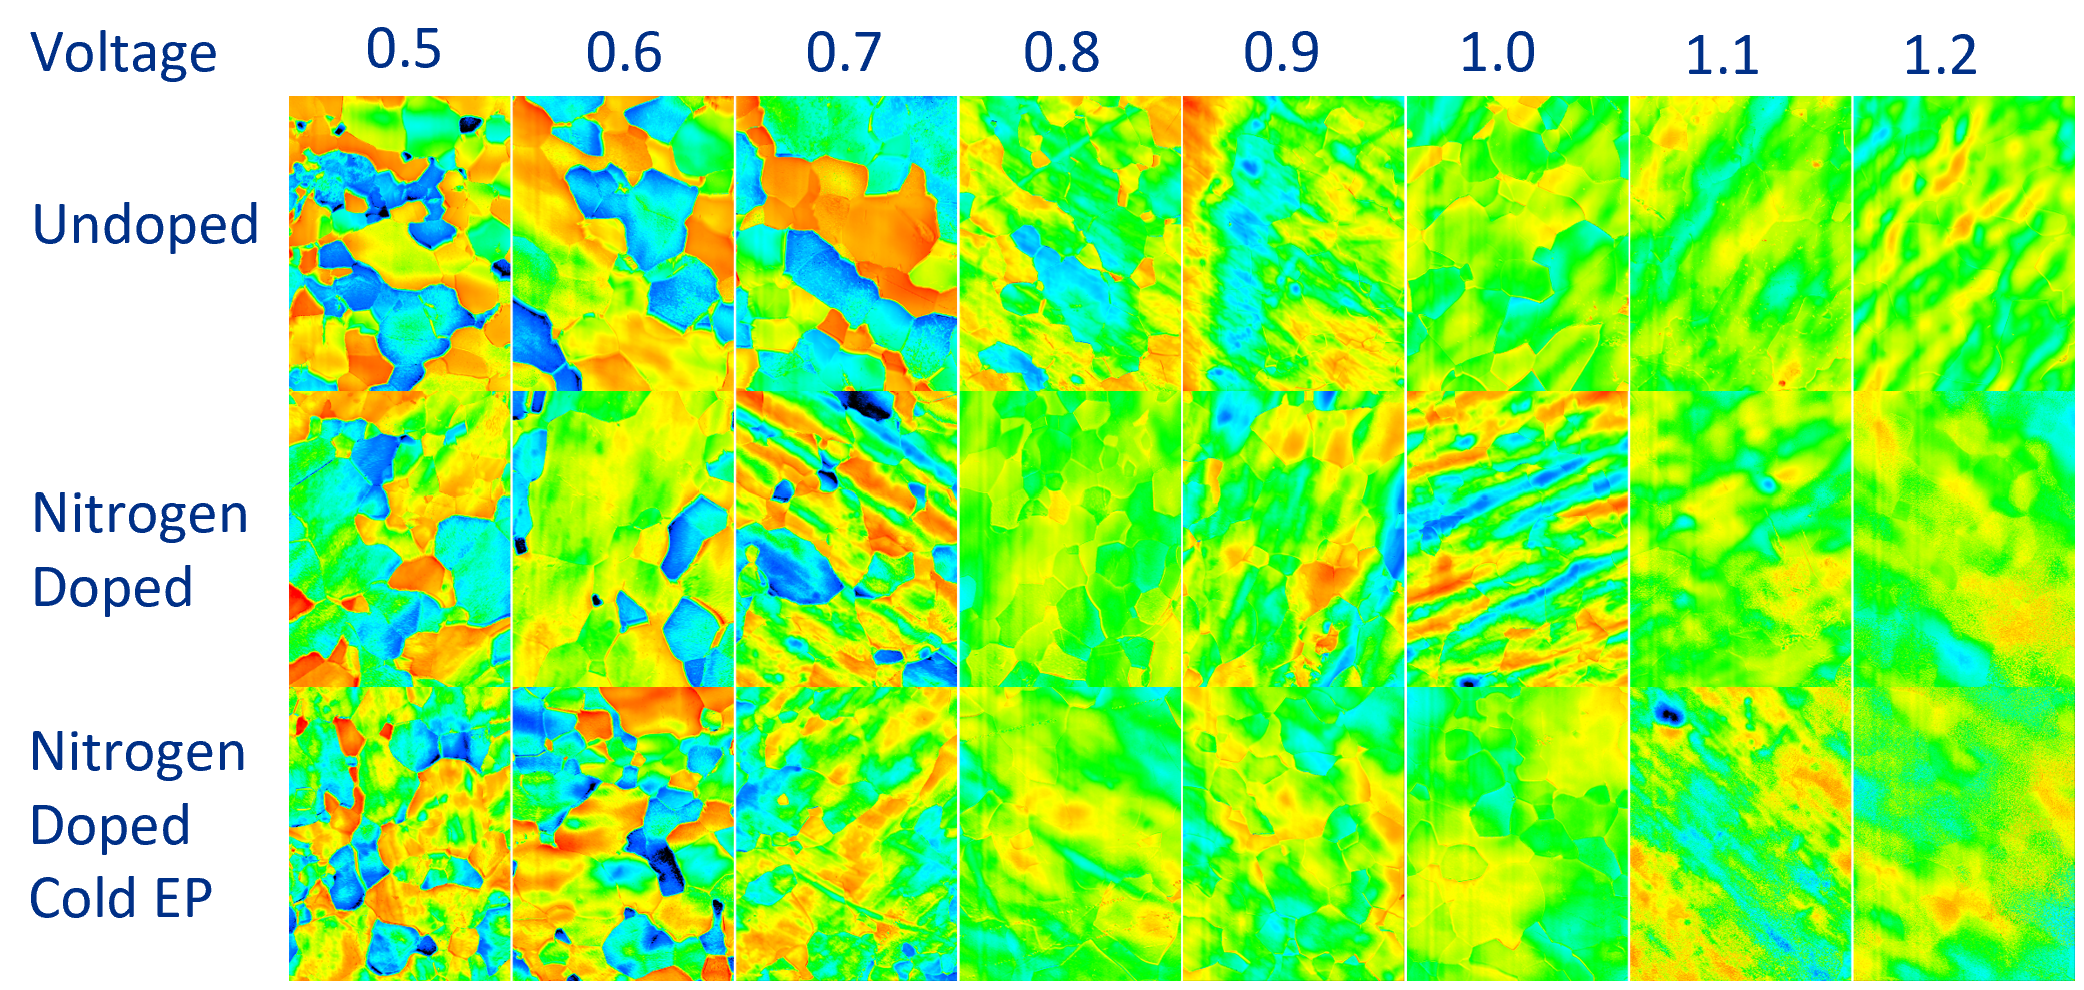
\includegraphics[width=\textwidth]{../figures/surface_maps.png}
    \caption{The surface height maps of Nb samples electropolished at different voltages and temperatures.}
\end{figure}

\section{Oxide Film Formation During Niobium Electropolishing}

The dissolution of niobium is caused by its reaction with HF and its ions in the electrolyte. However, before the niobium can be dissolved it must be oxidized. When the rate of oxidation exceeds the maximum rate of dissolution by HF, limited by diffusion of HF to the electrode surface, niobium oxides can form on the surface. The idea of a compact oxide film present during electropolishing is not a new one.\cite{Tian_2008,tian2008novel} Theories such as the point defect model have been used to explain the behavior of niobium and other pasivating metals\cite{bojinov1997ability, girginov2008conduction, bojinov2003evidence, macdonald1990theory, macdonald1992steady} Ranjith, et. al. propose a reaction model for niobium involving two intermediate adsorbed oxides, Nb\textsuperscript{2+} and Nb\textsuperscript{5+} and using this model qualitatively predict the impedance behavior in both the active and passive regions including the negative differential resistance which we have reported in our own measurments. The model, however, still deviates from the measured EIS spectrum by a significant amount.\cite{ranjith2018anodic}

When oxides begin to form on the surface, they do not cover the entire surface instantaneously. Due to slight differences in the oxidation reaction activation energy across the surface, caused by differing grain orientations, surface defects, and the local curvature, the oxide forms preferentially in certain areas. The surface has a mixed oxide with a certain fraction covered by Nb\textsubscript{2}O\textsubscript{5}, NbO, and Nb. As the surface potential is increased a larger portion of the electrode is covered by Nb\textsubscript{2}O\textsubscript{5}. Once the entire surface is covered, the dissolution rate of the surface becomes homogeneous and polishing can occur. This effect can be seen in \ref{fig:surface_maps} when the surface morphology changes from etching to polishing.


\section{Generalized Distribution of Relaxation Times}
\label{sec:org7d749e2}

The distribution of relaxation times is a flexible and general method that can be used to model complex impedance spectrum and extract useful information without the use of a pre-defined circuit model. In our study, we use this method to measure the changes on the niobium electrode as the polishing voltage is increased.

Traditional distribution of relaxation time analysis is based on a circuit model perspective on the electrochemical system. This perspective assumes the electrode is described by a series of voigt circuits, a resistor and a capacitor connected in parallel. By adding an infinite number of infinitesimal voigt elements, any arbitrary capacitive impedance can be described. The distribution of voigt elements is described by the distribution of relaxation times function.

\begin{flalign}
  \label{eq:Zrc}
  Z_{RC}\left(\omega\right) &= \frac{R}{1+j\omega R C}\\
  Z_{voigt}\left(\omega\right) &= R_{s} + \sum_{n=1}^{N} \frac{R_n}{1 + j \frac{\omega}{\omega_n}}\\
  Z_{DRT}\left(\omega\right) &= R_{s} + \int_{0}^{\infty} \frac{G(\omega_0) d \omega_0}{1 + j \frac{\omega}{\omega_0}}
\end{flalign}

This model is sufficient to describe any capacitive-like processes with positive real impedance and negative imaginary impedance. However, this does not encompass all possible behaviors of electrochemical systems. The impedance of electrochemical systems can exist in all four quadrants of the complex impedance plane. For example, as seen in figure \ref{fig:nyquistplot}, for Nb electropolishing the low frequency impedance loop curls to the left at \qty{0.86}{\volt}. We also observe an inductive mid-frequency loop as seen in figure \ref{fig:nyquistplot} when the voltage is \qty{0.78}{\volt} and \qty{0.86}{\volt}. These features cannot be explained using the traditional distribution of relaxation times.

To explain these different behaviors it is more intuitive to abandon the circuit model perspective of the electrode and instead consider the electrode reaction as a dynamical system. The electrochemical process can be described by a state vector whose evolution over time is described by a system of first order differential equations. Wu, et. al show that for a small perturbation, the impedance spectrum of such a system can always be represented as a sum of voigt-like elements given that both positive and negative capacitance and resistance are allowed.\cite{wu1998investigation, wu1999general}

\begin{flalign}
    \label{eq:gDRT}
    Z_{F}\left(\omega\right) &= R_{t} + \sum_{n=1}^{N} \frac{k_{n}}{j \omega - s_{n}} \\
    Z_{gDRT}\left(\omega\right) &= R_{t} + \int_{-\infty}^{\infty} \frac{k\left(s\right) ds}{j\omega - s} \\
    k\left(s\right) &= \omega_0 G\left(\omega_0\right) \\
    s &= -\omega_0 \\
    Z_{gDRT}\left(\omega\right) &= R_{t} + \int_{-\infty}^{\infty} \frac{G\left(\omega_0\right) d\omega_0}{1 + j\frac{\omega}{\omega_0}}
\end{flalign}

If we let $s_{i} = \frac{-1}{R_i C_i}$ and $k_{i} = \frac{1}{C_i}$ we see that this equation describes a classical voigt element. However, in this equation the constants $s_{i}$ and $k_{i}$ can take on both positive and negative values. We can take an infinite number of these voigt-like elements and add them together with the caviat that their sum converges to a finite impedance in the same way as the derivation of the classical DRT function, the only difference being the distribution spans both positive and negative frequencies and the function $G\left(omega_0\right)$ is free to take both positive and negative values. By generalizing the DRT method in this manner, it can in principle fit any linear time-invariant electrochemical system.



\section{Distribution of Relaxation Times of Niobium During Electropolishing}



\begin{figure}[t]
  \label{fig:bodeplot}
  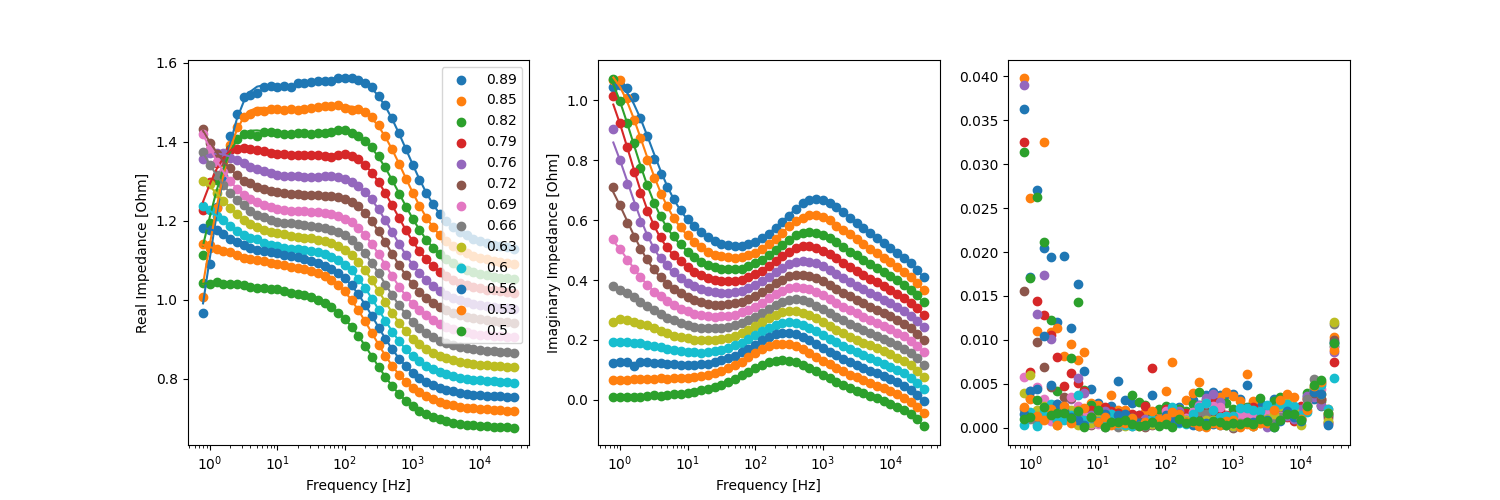
\includegraphics[width=\textwidth]{../figures/bodeplot.png}
  \caption{The complex impedance of Nb in electropolishing electrolyte measured using EIS. Each curve is offset from zero.}
\end{figure}

\begin{figure}[t]
  \label{fig:gamma}
  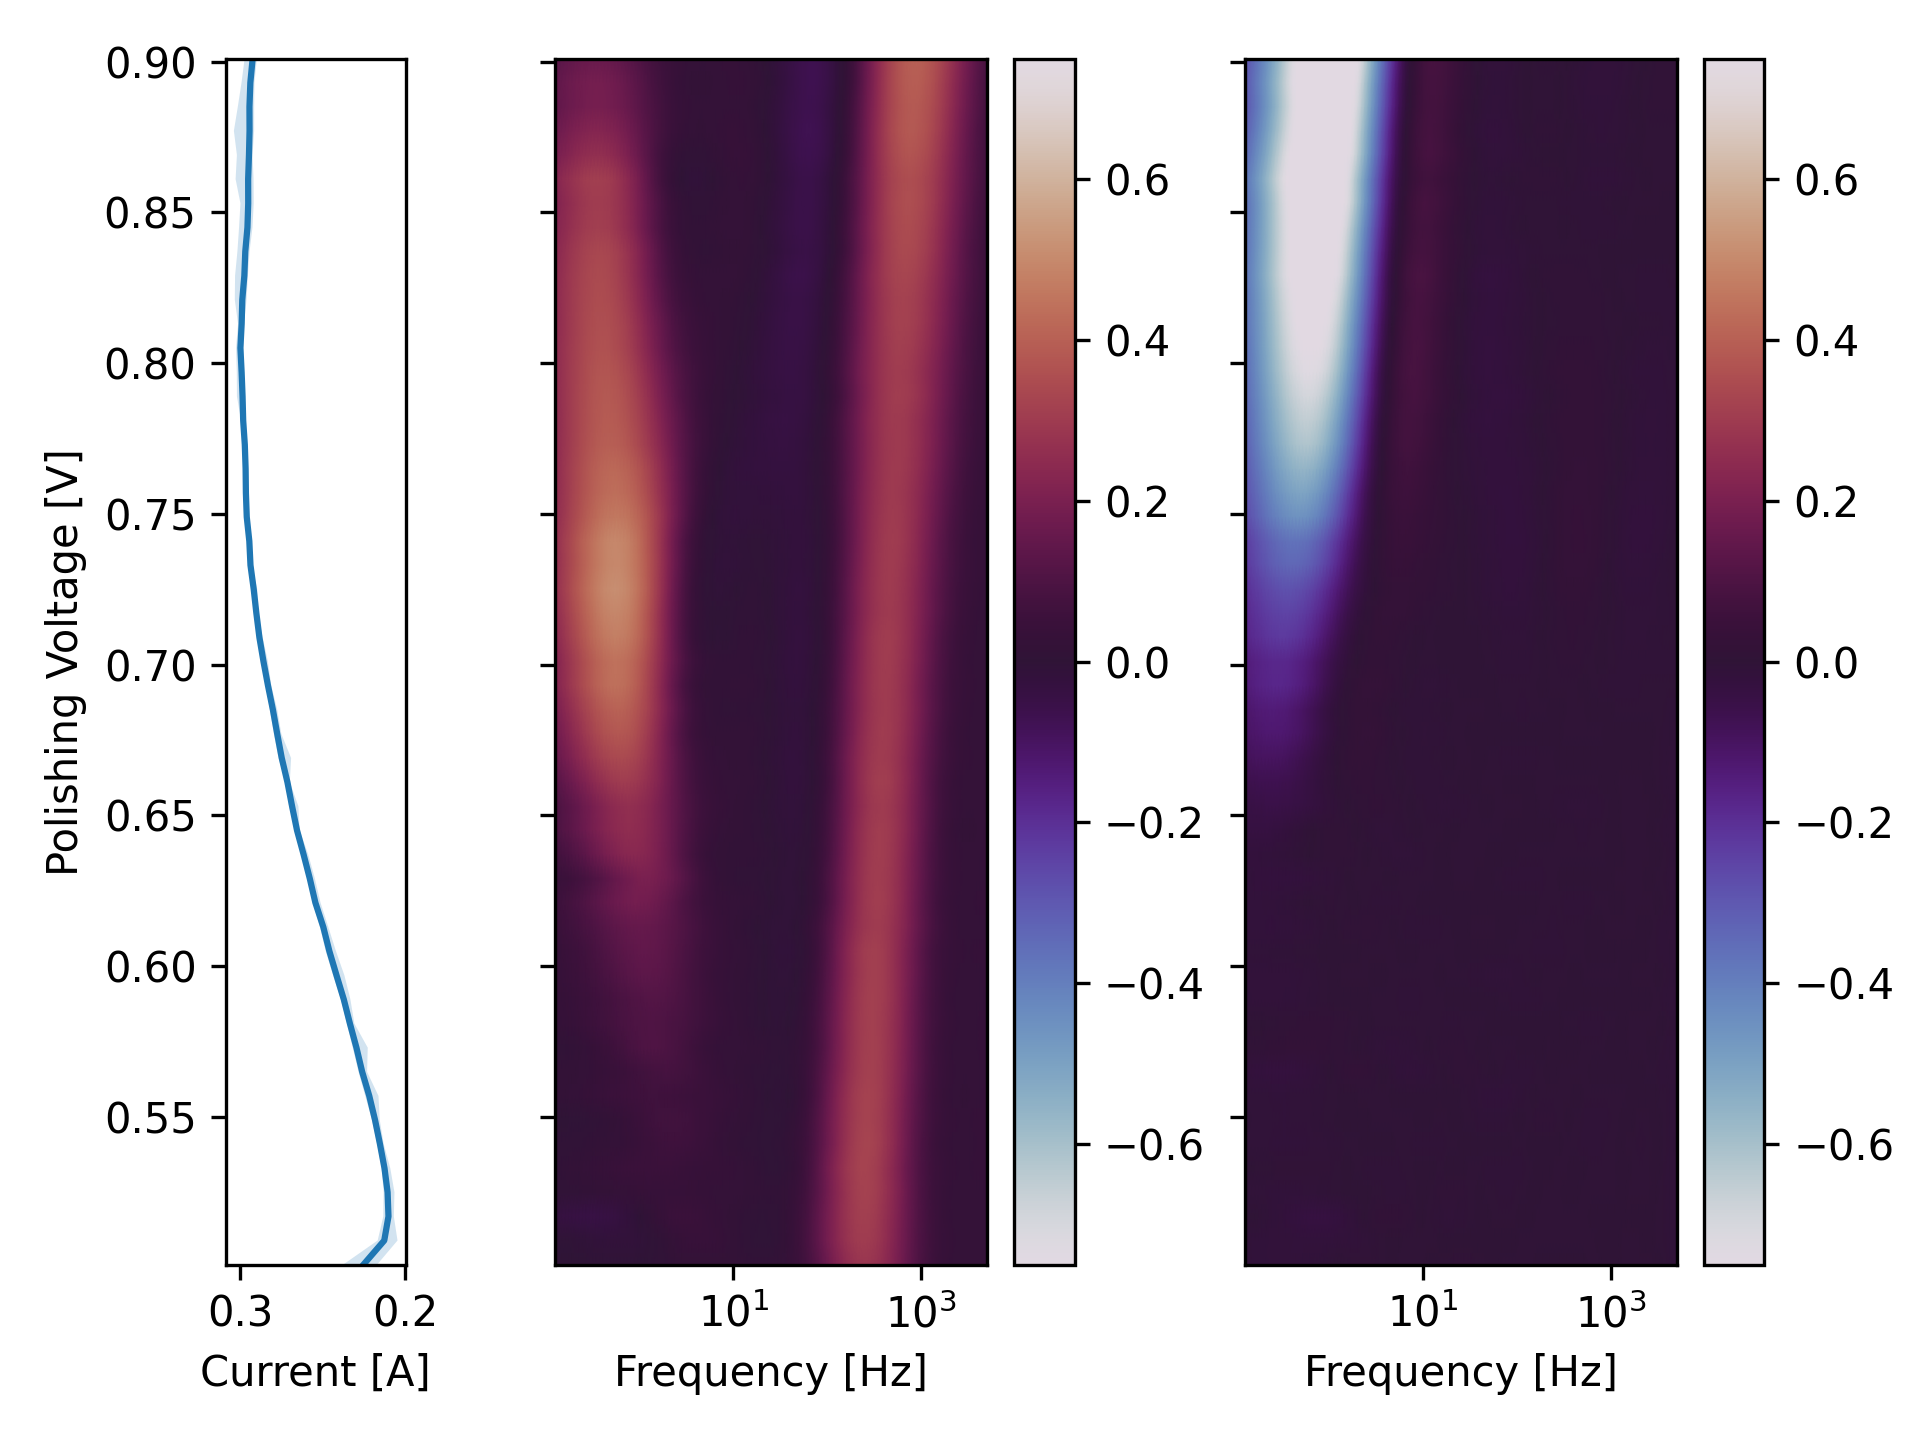
\includegraphics[width=\textwidth]{../figures/gamma.png}  
  \caption{The Distribution of relaxation times calculated from the EIS impedance data for each of the measured potentials. The current-voltage curve is shown in the graph on the left.}
\end{figure}

Using the generalized DRT method, we are able to fit the Nb impedance spectrum across all frequencies including the inductive mid-frequency loop and the low frequency loop as seen in figure \ref{fig:bodeplot}. From figure \ref{fig:gamma} we can see that there are three prominent peaks in the distribution of relaxations times. The peak centered around \qtyrange{100}{1000}{\hertz} corresponds to the electric double layer capacitance. The center of this peak shifts to the right linearly with the polishing voltage. This shows that the relaxation time of the electric double layer follows an Arrhenius type relation.

The two other peaks centered around \qty{10}{\hertz} most likely correspond to the oxide layer. This low frequency peak gets more pronounced at higher voltages which indicates greater electrical impedance due to the oxide film. Around \qty{0.75}{\volt} the third peak appears in the negative \qty{10}{\hertz} region. This peak indicates that the oxide film is blocking the current flow leading to a negative current-voltage relationship.



\section{Discussion}

Comparing figure \ref{fig:gamma} to the electropolished samples shown in figure \ref{fig:surface_maps} we can see that the appearance of the third peak coincides with a significant change in the surface of the electropolished niobium. The surface goes from an etched surface with facets and large grain boundary steps to a much more polished finish. We theorize that this transition is caused by the stabilization of the oxide film which occurs when the HF is depleted on the niobium electrode surface and the surface oxide transitions from a thin non-homogeneous layer to a thick homogeneous one. Since the oxide film is homogeneous, the effects of grain orientation on the dissolution reaction are eliminated. The result is a smoothing effect on the niobium. At polishing voltages below this critical voltage, the oxide film is too thin or does not cover the entire niobium surface, which leads to etching.

It is much more difficult to control the polishing voltage when eletcropolishing cavities compared to small scale samples. This is due to the much larger current and more complex geometry of the cavity and cathode. Currently, cavity electropolishing machines do not employ a reference electrode and instead only set a fixed voltage between the anode and cathode. This means that cathode losses and ohmic losses in the electrolyte can significantly alter the polishing potential and even create a non-homogeneous potential distribution over the surface of the cavity. This is why etching can occur even when applying much higher potentials typically used during cavity EP.

To combat the uncertainty of electropolishing cavities it may be possible to apply EIS measurements in the production environment. This would allow for a live diagnostic of the polishing conditions inside the cavity without interfering with the regular EP workflow. This information can be used to tweak the EP parameters such as voltage and temperature to ensure that the cavity is in an optimal polishing regime. Using this technique it may be possible to electropolish more complex cavity geometries such as quarter-wave and half-wave geometries.



\section{Conclusion}
\label{sec:org57282ed}
In this study we have shown that the etching phenomenon seen in electropolished SRF cavities is caused by insufficient polishing voltage. Niobium polished below a critical voltage will experience etching whereas niobium polished above this voltage will experience smoothing. We theorize that the cause of this change in surface finish is a transition from a partially formed niobium oxide film to a fully formed, stable oxide film. This theory is evidenced by measurements of the niobium electropolishing impedance spectrum over a range of polishing voltages. The impedance spectrum indicates the presence of a blocking mechanism that limits the current. This blocking mechanism is most likely caused by the oxide film which forms when HF is depleted near the niobium surface and the oxidation rate exceeds the rate of dissolution by HF.


\section{Supplemental Information}
\label{sec:sup}

This Supplemental section will cover the mathematical process of calculating the generalized DRT from experimental measurements of the impedance spectrum. To find the DRT function numerically, we must first discretize the function using a finite set of basis functions which will approximate the continuous DRT function. This is done by first transforming the problem into the much more natural log space. For a chosen basis function, the integral can then be calculated numerically and the problem is then transformed into a simple case of linear regression. We must also apply a normalization procedure to our regression to prevent overfitting.

\subsection{Discretizing the Integral of the Generalized DRT Function in Log Coordinates}

It is necessary to discretize the DRT function in the log based coordinate system since EIS measurements are typically performed over many orders of magnitude in frequency. Otherwise, the computational accuracy will be too low at the low frequencies, or too high at the high frequencies. However, this procedure is more challenging for the generalized DRT model, since the integral spans both positive and negative values. To solve this problem we must separate the integral in equation~\ref{eq:gDRT} into the sum of two integrals each integrating over one side of the real axis. After a change of variables and reversing the direction of integration we can substitute $G\left(\omega_0\right)$ with a piece wise fit function $\gamma_{\pm}\left(\ln\omega_0\right)$.



\begin{flalign}
  Z_{gDRT} =& R_{t} + \int_{-\infty}^{0}\frac{G(\omega_0)d\omega_0}{1 + j \frac{\omega}{\omega_0}} + \int_{0}^{\infty}\frac{G(\omega_0)d\omega_0}{1 + j \frac{\omega}{\omega_0}}\\
  Z_{gDRT} =& R_{t} + \int_{0}^{\infty}\frac{G(\omega_0)d\omega_0}{1 + j \frac{\omega}{\omega_0}} + \frac{G(-\omega_0)d\omega_0}{1 - j \frac{\omega}{\omega_0}}\\
  G\left(\omega_0\right) d\omega_0 =& \begin{cases}
    \gamma_+\left(\ln\omega_0\right) d\ln\omega_0 & \omega_0 \ge 0 \\
    \gamma_-\left(\ln-\omega_0\right) d\ln\omega_0 & \omega_0 \le 0 \\
  \end{cases}\\
  Z_{gDRT} =& R_{t} + \int_{-\infty}^{\infty}\frac{\gamma_+\left(\ln\omega_0\right) d\ln\omega_0}{1 + j \frac{\omega}{\omega_0}} + \frac{\gamma_-\left(\ln\omega_0\right) d\ln\omega_0}{1 - j \frac{\omega}{\omega_0}}
\end{flalign}

To solve for the functions \(\gamma_{\pm}(\ln\omega_0)\) numerically we approximate the function using a basis function $\phi_n\left(\ln\omega_0\right)$.

\begin{flalign}
  \gamma_{\pm}(\ln\omega_0)&\approx\sum_{n=1}^{N}x^{\pm}_{n}\phi_{n}(\ln\omega_0)\\
  Z_{gDRT} =& R_{t} + \int_{-\infty}^{\infty}\sum_{n=1}^{N}\frac{x^{+}_{n}\phi_{n}(\ln\omega_0)d\ln\omega_0}{1 + j \frac{\omega}{\omega_0}} + \sum_{n=1}^{N}\frac{x^{-}_{n}\phi_{n}(\ln\omega_0)d\ln\omega_0}{1 - j \frac{\omega}{\omega_0}}
\end{flalign}

Using algebraic manipulation and a change of variables, the integral can be separated into a real part and an imaginary part.

\begin{flalign}
  x_n^{re} =& x_n^+ + x_n^-\\
  x_n^{im} =& x_n^+ - x_n^-\\
  Z_{gDRT} =& R_{t} + \sum_{n=1}^{N}x^{re}_{n} \int_{-\infty}^{\infty} \frac{\phi_{n}(\ln\omega_0)d\ln\omega_0}{1 + \left(\frac{\omega}{\omega_0}\right)^2} + j \sum_{n=1}^{N}x^{im}_{n} \int_{-\infty}^{\infty} \frac{\frac{\omega}{\omega_0}\phi_{n}(\ln\omega_0)d\ln\omega_0}{1 + \left(\frac{\omega}{\omega_0}\right)^2}
\end{flalign}

The impedance at a frequency $\omega = \omega_m$ is a linear function of the values of $x^{re}_n$ and $x^{im}_n$.

\begin{flalign} \label{eq:A}
  Z_{gDRT}\left(\omega_m\right) =& R_{t} + \sum_{n=1}^{N} x^{re}_{n} A^{re}_{n,m} + \sum_{n=1}^{N} x^{im}_{n} A^{im}_{n,m}\\
  A^{re}_{n,m} =& \int_{-\infty}^{\infty} \frac{\phi_{n}(\ln\omega_0)d\ln\omega_0}{1 + \left(\frac{\omega_m}{\omega_0}\right)^2}\\
  A^{im}_{n,m} =& \int_{-\infty}^{\infty} \frac{\frac{\omega_m}{\omega_0}\phi_{n}(\ln\omega_0)d\ln\omega_0}{1 + \left(\frac{\omega_m}{\omega_0}\right)^2}
\end{flalign}

Given a set of M experimentally measured impedance data points, $\mathbf{Z_{exp}} = \left[Z_1, \ldots, Z_M\right]$ at frequencies $\mathbf{\omega} = \left[\omega_1, \ldots, \omega_M\right]$ we can find the values of $x^{re}_n$ and $x^{im}_n$ using linear regression.

\begin{flalign}\label{eq:Zmatrix}
  \min_{\mathbf{x^{re}},\mathbf{x^{im}}}\lVert\mathbf{Z_{gDRT}}-\mathbf{Z_{exp}}\rVert = \min_{\mathbf{x^{re}},\mathbf{x^{im}}}\left(\lVert \mathbf{x^{re}} \mathbf{A^{re}} - Re\left(\mathbf{Z_{exp}}\right) \rVert + \lVert \mathbf{x^{im}} \mathbf{A^{im}} - Im\left(\mathbf{Z_{exp}}\right) \rVert \right)
\end{flalign}

\subsection{Normalization}

When finding the DRT function from experimental data, a normalization method is required to prevent overfitting. In this study we use a modified Tikhonov regularization, based on the work of Wan, et. al.~\cite{wan2015influence}, that penalizes the derivatives of the DRT function. This has the effect of smoothing the function and eliminating oscillations caused by overfitting. With the regularization term added the objective becomes to minimize the residuals and the normalization term together. 

\begin{flalign}
  \min_{\mathbf{x^{re}},\mathbf{x^{im}}}\left(\lVert \mathbf{x^{re}} \mathbf{A^{re}} - Re\left(\mathbf{Z_{exp}}\right) \rVert + \lVert \mathbf{x^{im}} \mathbf{A^{im}} - Im\left(\mathbf{Z_{exp}}\right) \rVert + \mathbf{x^{re} M x^{re}}^T + \mathbf{x^{im} M x^{im}}^T \right)
\end{flalign}

The matrix $\mathbf{M}$ is calculated by integrating the square of the derivatives of the test functions, $\phi_n\left(\omega_0\right)$. Calculating the zeroth derivative, i.e. the function itself, is equivalent to standard Tikhonov regularization. The strength of the regularization is controlled by multiplying by a constant $\lambda_k$, where $k$ is the k-th derivative of the test functions.

\begin{flalign}
  (\mathbf{M}_{k})_{n,m} =& \int_{-\infty}^{\infty} \frac{d^{k}\phi_{n}}{dln\tau^{k}} \frac{d^{k}\phi_{m}}{dln\tau^{k}} dln\tau\\
  \mathbf{M} =& \sum_{k=0}^{K}\lambda_{k}\mathbf{M}_{k}
\end{flalign}

The optimum values of \(\lambda_k\) are difficult to find mathematically, so values were manually adjusted up to $k=2$ to maximize the fitting strength without sacrificing the accuracy of the fit. Mathematical heuristics such as the L-curve, cross-validation, Fourier transform\cite{BOUKAMP201712} or Bayesian methods\cite{ciucci2015analysis}.





\subsection{Basis Function}
\label{sec:org8198a5a}

The choice of basis function is quite arbitrary as long as the resulting function space is large enough to contain the exact solution for the DRT function. However, in practice the basis function has a large impact on the number of parameters required and the level of regularization required. The basis function should also be relatively easy to compute using a computer to speed up the computation and differentiable so that the regularization matrix can be calculated. A natural choice is to use the log Gaussian, which has been shown to be effective at fitting the DRT function for several kinds of impedance systems\cite{wan2015influence}.

\begin{flalign}
  \phi_{n}(ln\omega) &= \frac{1}{\sigma\sqrt{2\pi}}e^{-\left(\frac{ln\omega_0-ln\omega_{n}}{\sigma\sqrt{2}}\right)^2}
\end{flalign}

Plugging this test function into equation~\ref{eq:A} produces two integrals for $A^{re}$ and $A^{im}$.

\begin{flalign}
  A^{re}_{n,m} =& \frac{1}{\sigma\sqrt{2\pi}} \int_{-\infty}^{\infty} \frac{e^{-\left(\frac{ln\omega_0-ln\omega_{n}}{\sigma\sqrt{2}}\right)^2} d\ln\omega_0}{1 + e^{2\left(\ln\omega_m - \ln\omega_0\right)}}\\
  A^{im}_{n,m} =& \frac{1}{\sigma\sqrt{2\pi}} \int_{-\infty}^{\infty} \frac{e^{\ln\omega_m-\ln\omega_0} e^{-\left(\frac{ln\omega_0-ln\omega_{n}}{\sigma\sqrt{2}}\right)^2} d\ln\omega_0}{1 + e^{2\left(\ln\omega_m - \ln\omega_0\right)}}
\end{flalign}




\bibliography{generalized_DRT}


\end{document}